\section{Ergebnis}

In dieser Arbeit wurde eine Nagios-Umgebung entwickelt, die eine umfassende Überwachung von \gls{OracleUCM} ermöglicht.
Das Ergebnis lässt sich im Webinterface von Nagios betrachten, siehe Abbildung \ref{nweb}.

%Die in dieser Arbeit erbrachte Lösung ermöglicht die Überwachung der in Kapitel \ref{elemente} genannten Elemente.
% die Umsetzung der Aufgabenstellung  liefert das Produkt
%das aus der Aufgabenstellung resultierende Ausgabe beinhaltet folgende Ausgabe.
%Das Ergebnis lässt sich im 

%\begin{itemize}
%\item Vllt. Übersicht wie was überwacht wird
%\item Screenshots von Nagios
%\item Exportierfähigkeit, was muss alles auf dem Live-Nagios Server gemacht werden
%\end{itemize}

\begin{figure}[ht]
	\centering
	  \fbox{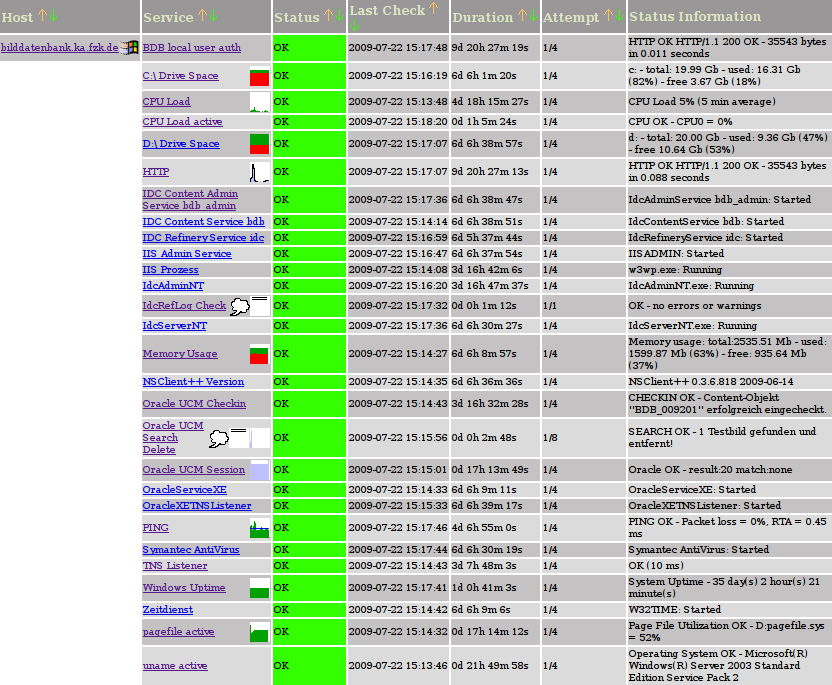
\includegraphics[width=0.93\textwidth]{bilder/demo.png}}
		\caption{Webinterface von Nagios}
		\label{nweb}
\end{figure}

Die einzelnen Elemente der Überwachung lassen sich mit Ausnahme der Benutzersimulation durch Konfiguration von bereits vorhandenen Nagios-Plugins überprüfen.
Bei dieser Konfiguration müssen die bereits im Kapitel \ref{monitor} erörterten Gesichtspunkte wie Netzwerkabhängigkeiten, -belastung und sichherheitstechnische Aspekte bedacht werden.
Gerade bei der Verwendung von Benutzerinformationen zur Authentifizierung ist es notwendig zu überprüfen, ob die Informationen als Klartext oder verschlüsselt übertragen werden.
Diese Überprüfung lässt sich durch Programme, wie Wireshark\footnote{Quelle: \url{http://www.wireshark.org/}}, durchführen.
Wireshark protokolliert alle ein- und ausgehenden Netzwerkverbindungen mit.
Bei einer Ausführung eines Checks mit einem Nagios-Agenten, welcher keine Verschlüsselung ermöglicht, lassen sich Informationen abfangen.
\begin{figure}[ht]
	\centering
	  \fbox{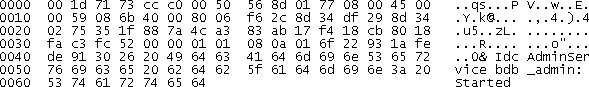
\includegraphics[width=0.85\textwidth]{bilder/klartext.png}}
		\caption{Klartext im Mitschnitt}
		\label{klartxt}
\end{figure}

Währenddessen bei Agenten mit Verschlüsselung sich aus mitgeschnittenen Daten keine brauchbaren Informationen herauslesen lassen.
\begin{figure}[ht]
	\centering
	  \fbox{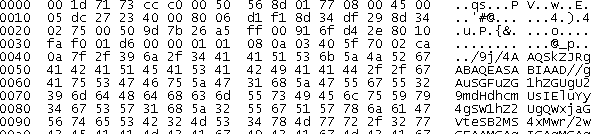
\includegraphics[width=0.85\textwidth]{bilder/ssl-text.png}}
		\caption{Verschlüsselte Übertragung von Informationen}
		\label{ssltxt}
\end{figure}

Die durch die einzelnen Plugins gesammelten Informationen lassen sich zusätzlich im Detail aufrufen:

\begin{figure}[ht]
	\centering
	  \fbox{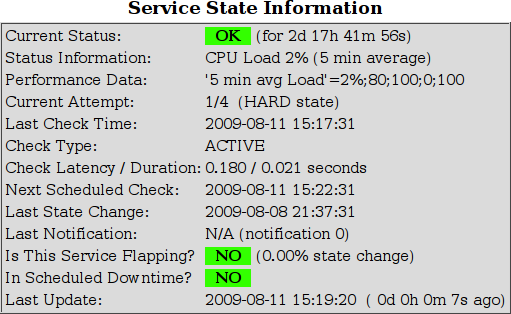
\includegraphics[width=0.68\textwidth]{bilder/cpu-load2.png}}
		\caption{Details der Prozessorauslastung}
		\label{cpuload}
\end{figure}


Wie in Kapitel \ref{performanz} erwähnt können zusätzliche Add-ons installiert werden, die die von Nagios eingesammelten Informationen visualisieren.
Dazu kann der verbreitete Nagios Grapher der Firma NETWAYS\footnote{Quelle: \url{http://www.netways.de/de/produkte/nagios_addons/nagiosgrapher/}} verwendet werden.

Dieser wertet die Performanzinformationen der Nagios-Plugins aus und erstellt davon Graphen.

\begin{figure}[ht]
	\centering
	  \fbox{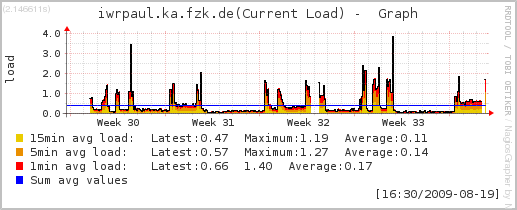
\includegraphics[width=0.85\textwidth]{bilder/iwrp-load.png}}
		\caption{Darstellung der Prozessortauslastung}
		\label{iwrpload}
\end{figure}

Die zeitliche Auflösung kann zwischen Minuten und Jahren dynamisch gewählt werden, um eventuelle Tendenzen zu erkennen.
Die Anzeige der Arbeitsspeicherauslastung über einen längeren Zeitraum kann helfen speicherintensive Programme zu entdecken.
\begin{figure}[ht]
	\centering
	  \fbox{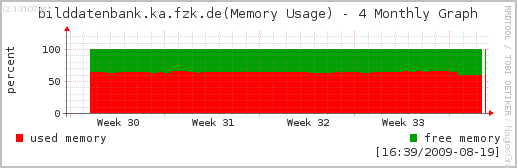
\includegraphics[width=0.85\textwidth]{bilder/bdbd-mem4.png}}
		\caption{Arbeitsspeicherauslastung über vier Monate}
		\label{bdb-mem}
\end{figure}


